
\begin{figure}[H]
  {
    \setlength{\tabcolsep}{3.0pt}
    \setlength\cmidrulewidth{\heavyrulewidth} % Make cmidrule = 
    \begin{adjustbox}{height=5cm,center}
      \footnotesize
      \begin{tabular}{ll}

        \makecell[l]{
\icode{.BYTE \$00,\$01,\$00,\$FF}\\
\icode{.BYTE \$FF,\$00,\$01,\$00}
} & \makecell[l]{

\includegraphics[width=1.3cm]{src/patterns/pixels/pixel_pattern7_0.png}%
} \\
        \midrule

        \makecell[l]{
\icode{.BYTE \$00,\$02,\$00,\$FE}\\
\icode{.BYTE \$FE,\$00,\$02,\$00}
} & \makecell[l]{

\includegraphics[width=1.3cm]{src/patterns/pixels/pixel_pattern7_1.png}%

\includegraphics[width=1.3cm]{src/patterns/pixels/pixel_pattern7_2.png}%
} \\
        \midrule

        \makecell[l]{
\icode{.BYTE \$00,\$03,\$00,\$FD}\\
\icode{.BYTE \$FD,\$00,\$03,\$00}
} & \makecell[l]{

\includegraphics[width=1.3cm]{src/patterns/pixels/pixel_pattern7_3.png}%

\includegraphics[width=1.3cm]{src/patterns/pixels/pixel_pattern7_4.png}%

\includegraphics[width=1.3cm]{src/patterns/pixels/pixel_pattern7_5.png}%
} \\
        \midrule

        \makecell[l]{
\icode{.BYTE \$00,\$04,\$00,\$FC}\\
\icode{.BYTE \$FC,\$00,\$04,\$00}
} & \makecell[l]{

\includegraphics[width=1.3cm]{src/patterns/pixels/pixel_pattern7_6.png}%

\includegraphics[width=1.3cm]{src/patterns/pixels/pixel_pattern7_7.png}%

\includegraphics[width=1.3cm]{src/patterns/pixels/pixel_pattern7_8.png}%

\includegraphics[width=1.3cm]{src/patterns/pixels/pixel_pattern7_9.png}%
} \\
        \midrule

        \makecell[l]{
\icode{.BYTE \$00,\$05,\$00,\$FB}\\
\icode{.BYTE \$FB,\$00,\$05,\$00}
} & \makecell[l]{
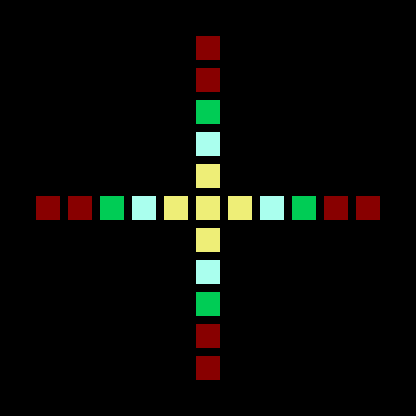
\includegraphics[width=1.3cm]{src/patterns/pixels/pixel_pattern7_10.png}%
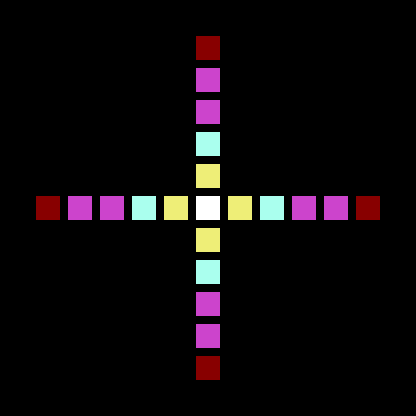
\includegraphics[width=1.3cm]{src/patterns/pixels/pixel_pattern7_11.png}%
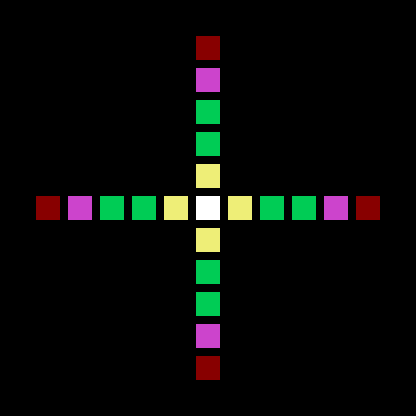
\includegraphics[width=1.3cm]{src/patterns/pixels/pixel_pattern7_12.png}%
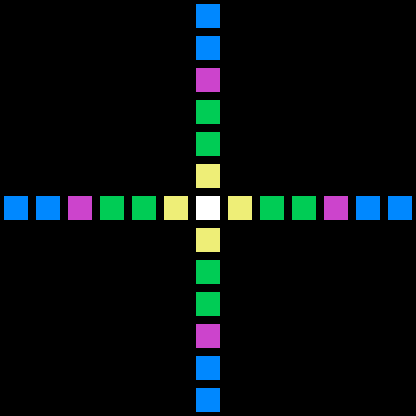
\includegraphics[width=1.3cm]{src/patterns/pixels/pixel_pattern7_13.png}%
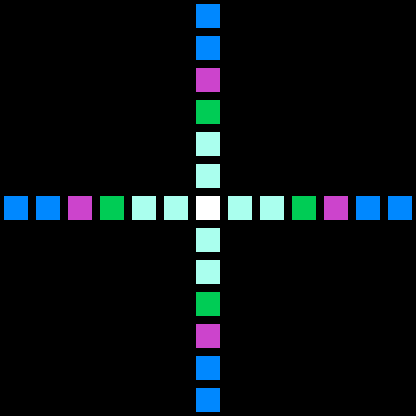
\includegraphics[width=1.3cm]{src/patterns/pixels/pixel_pattern7_14.png}%
} \\
        \midrule

        \makecell[l]{
\icode{.BYTE \$00,\$06,\$00,\$FA}\\
\icode{.BYTE \$FA,\$00,\$06,\$00}
} & \makecell[l]{
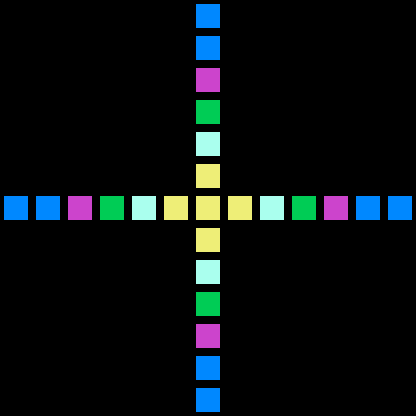
\includegraphics[width=1.3cm]{src/patterns/pixels/pixel_pattern7_15.png}%
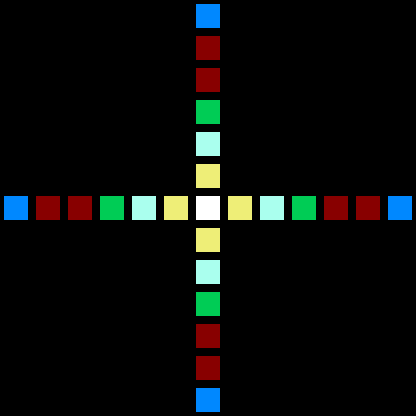
\includegraphics[width=1.3cm]{src/patterns/pixels/pixel_pattern7_16.png}%
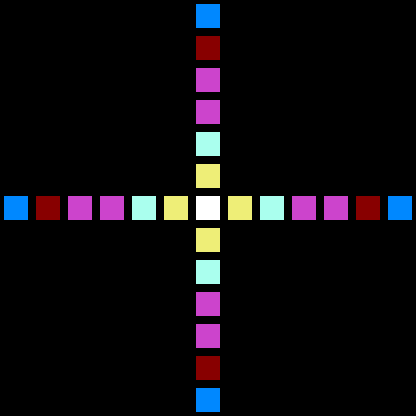
\includegraphics[width=1.3cm]{src/patterns/pixels/pixel_pattern7_17.png}%
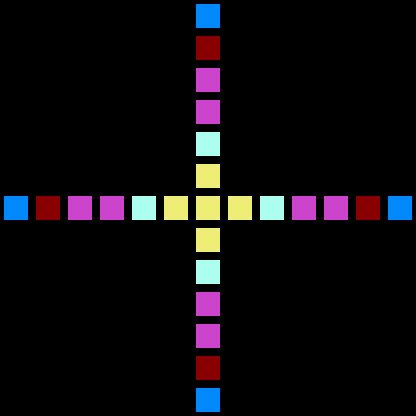
\includegraphics[width=1.3cm]{src/patterns/pixels/pixel_pattern7_18.png}%
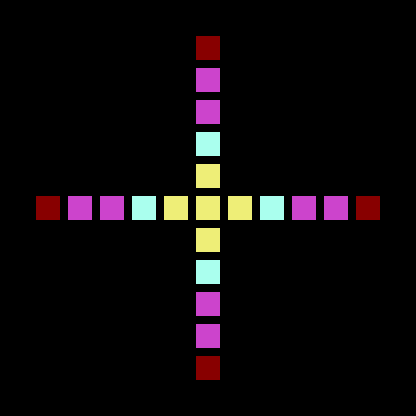
\includegraphics[width=1.3cm]{src/patterns/pixels/pixel_pattern7_19.png}%
} \\
        \midrule

        \makecell[l]{
\icode{.BYTE \$00}\\
\icode{.BYTE \$00}
} & \makecell[l]{
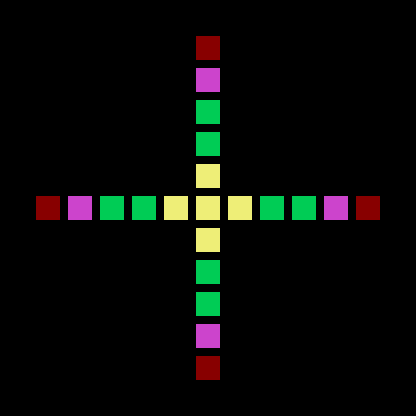
\includegraphics[width=1.3cm]{src/patterns/pixels/pixel_pattern7_20.png}%
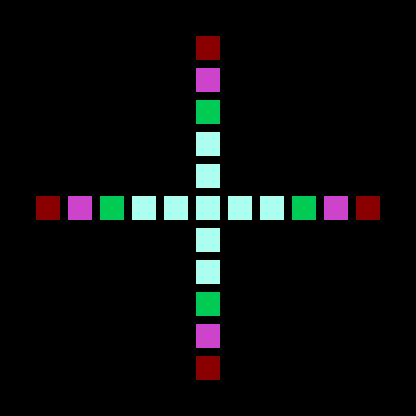
\includegraphics[width=1.3cm]{src/patterns/pixels/pixel_pattern7_21.png}%
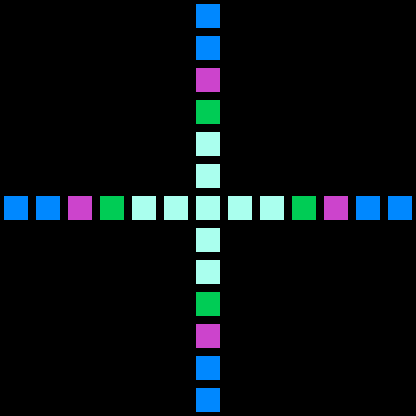
\includegraphics[width=1.3cm]{src/patterns/pixels/pixel_pattern7_22.png}%
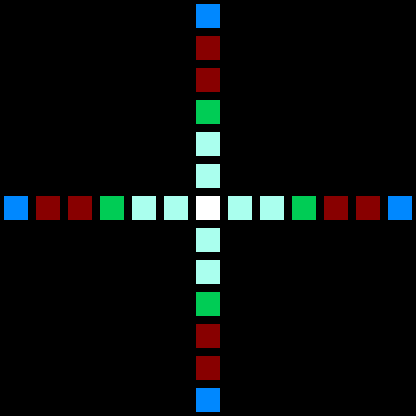
\includegraphics[width=1.3cm]{src/patterns/pixels/pixel_pattern7_23.png}%
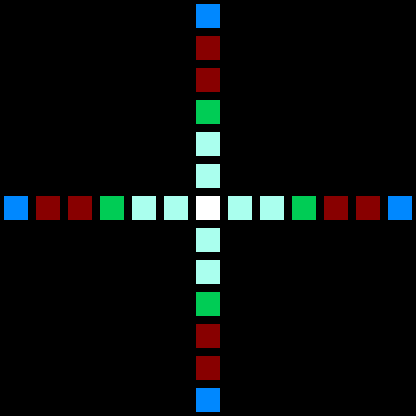
\includegraphics[width=1.3cm]{src/patterns/pixels/pixel_pattern7_24.png}%
} \\
        \midrule

      \end{tabular}
    \end{adjustbox}
  }\caption{The purpose of each of the oscillator values.}
\end{figure}
